% Sample file on how to use subfiles.
\documentclass[ExampleMasters.tex]{subfiles}

\begin{document}
\clearpage
\chapter{Steering Model (3 Seiten)}
\label{chap:steering_model}
There are two different controllers used to control the steerable axles of the dolly. One is used for low-speed and one for high-speed maneuvers. The main purpose of the low-speed controller is the reduction of off-tracking.
For the high-speed controller the aim is to reduce the rearward amplification.
\section{Low-Speed controller}
\label{sec:low-speed_controller}
The low-speed controller is implemented in path-distance domain $\eta$. The path-distance is calculated by integrating the forward speed $v_{x,1}(t)$. \\
The steering angle of the first axle of the dolly is calculated as follows: 
\begin{equation}
\delta_{31}(\eta)=k_1\delta_{11}(\eta-\eta_1)+k_2\Delta\psi_1(\eta-\eta_2)+k_3\Delta\psi_2(\eta-\eta_3)+k_4\Delta\psi_3(\eta-\eta_4)
\end{equation}

\label{eq:delta31_lowspeed}

The steering angle of the second axle of the dolly is calculated using the steering angle of the first dolly axle as follows:
\begin{equation}
\delta_{32}(\eta)=k_5\delta_{31}(\eta-\eta_5)
\end{equation}
\label{eq:delta32_lowspeed}

\begin{figure}[h]
	\centering
	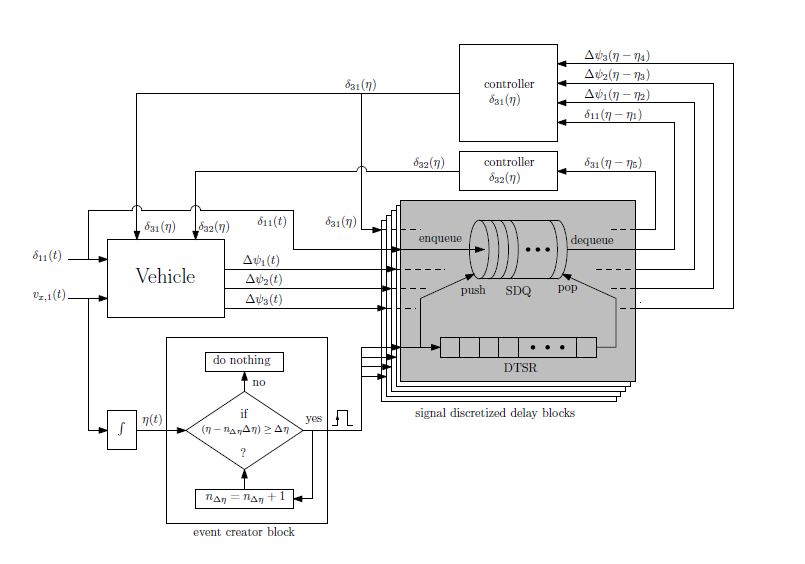
\includegraphics[width=1.0\linewidth]{figures/Low_speed_diagram}
	\caption[]{Controller implementation in the functional architecture \cite{Low-speed_paper}}
	
	\label{fig:low_speed_diagram}
\end{figure}

\begin{itemize}
	\item controller uses path-distance domain instead of time domain
\item path distance is calculated by integrating vx
\item optimization of gains using particle swarm optimization
\item path distance in time domain transformation needed
\end{itemize}

\subsection{Input parameters}
\label{sec:input_parameters_LS}

\begin{itemize}
	\item for delta 31: delta phi 1-3 (n) + delta11(n)
	\item for delta 32: delta31
\end{itemize}
\section{High-Speed controller}
\label{sec:high-speed_controller}
\begin{itemize}
\item The controller is implemented using a nonlinear inverse of a dynamic vehicle model.
\item same path of all units --> time delay of units considered
\item lateral acceleration of dolly(t) = lat. accel. of truck(t-tau)
\item modelica used because it can do inverse models
\item imported to simulink as a functional mock-up unit (FMU) using FMI-toolbox
\subsection{Input parameters}
\label{sec:input_parameters_HS}

\begin{itemize}
	\item ay3ref = delayed ay1
	\item ay3; delta11, vx
	\item derivative of delta11 needed for inversion operation
	\item explain feedback/inverse path
	
\end{itemize}

\end{itemize}
 \begin{figure}[h]
 	\centering
 	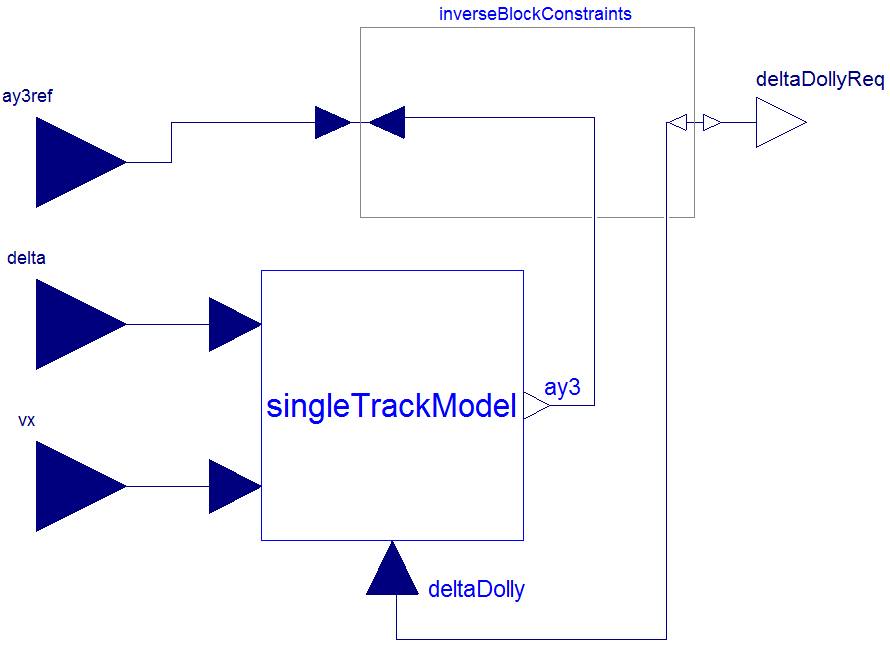
\includegraphics[width=1.0\linewidth]{figures/Inverse_of_A-double_single-track}
 	\caption[]{Inverse of the single track A-double model \cite{High-speed_paper}}
 
 	\label{fig:inverse_model}
 \end{figure}
 
\section{Overview of the model}
\label{sec:overview_of_the_model}
			
\begin{itemize}
	\item based on lit from MI-paper 
	\item overview graph of model
	\item single track model
	
	\item filtering of inputs?
	\item feedback-loop
	\item start condition
	\item what can be concluded with the model?
\end{itemize}



\section{Real-Time implementation}
\label{sec:real_time_implementation}

\begin{itemize}
	\item what had to be changed to allow for MABII execution?
	\item how will feedback loop be handled?
	item incorporate measurings?
	\item simulation step size?
	\item utilized computational method
\end{itemize}

\section{Interface with Real-Time environment}
\label{sec:interface_with_real_time}

\begin{itemize}
	\item capabilities of system (see section \ref{sec:maxi_capabilities})
	\item signals passed forward from environment + restriction
	
	\item actuator signals
	\item signal modification (correct frequency for CAN)
	\item safety flags/signals
	
\end{itemize}

\end{document}
